\documentclass{article}
\usepackage[letterpaper,body={6.3in,9.15in},top=.8in,left=1.1in]{geometry}
\usepackage{fancyvrb,color,gretl}
\usepackage{amsmath}
\usepackage{graphicx}
\usepackage[authoryear]{natbib}
\usepackage[pdftex,hyperfootnotes=false]{hyperref}

\definecolor{steel}{rgb}{0.03,0.20,0.45}

\hypersetup{pdftitle={kmeans},
            pdfauthor={Artur Tarassow and Allin Cottrell},
            colorlinks=true,
            linkcolor=blue,
            urlcolor=red,
            citecolor=steel,
            bookmarksnumbered=true,
            plainpages=false
          }

\setlength{\parskip}{1ex}
\setlength{\parindent}{0pt}
\setcounter{secnumdepth}{1}
\setcounter{tocdepth}{1}

\renewcommand{\floatpagefraction}{.8}

\newenvironment{funcdoc}
{\noindent\hrulefill\\[-12pt]}
{\medbreak}

\title{The \textsf{kmeans} addon}
\author{Artur Tarassow and Allin Cottrell}
\date{June 23, 2026}

\begin{document}
\maketitle

\section{Introduction}

In conjunction with gretl's built-in \texttt{kmeans} function this
package provides functionality to identify clusters in multidimensional
data using the $K$-means algorithm.  This algorithm divides a set of $m$
observations, each of dimension $n$, into disjoint clusters,
$C_i, i=1,\dots,K$. Each cluster is defined by its centroid, an
$n$-vector comprising the means of the variables for the observations it
includes. Useful references include \citet{hartigan-wong79} and
\citet[ch.\ 12]{ISL2e}.

The aim of $K$-means is to minimize a loss function, namely the total
distance between the data-points and their associated cluster
centroids. Most commonly the metric is squared Euclidean distance (sum
of squares of the distances in each of the $n$ dimensions) but other
metrics---such as Manhattan (sum of the absolute distances in each
dimension) or Chebyshev (greatest absolute distance in any
dimension)---are sometimes used.

In brief, here's the relationship between the built-in \texttt{kmeans}
function and the \texttt{kmeans} addon (with primary function
\dtk{kmeans_fit}). Built-in \texttt{kmeans} is fully specialized to
squared Euclidean distance, and employs a C-coded version of algorithm
ASA136 \cite{hartigan-wong79}, which is known to be particularly
efficient. The addon takes the squared Euclidean metric as default, and
in fact \dtk{kmeans_fit} calls built-in \texttt{kmeans} to solve the
basic $K$-means problem if that metric is in use. But the addon also
supports a variety of alternative metrics, and it provides tools to
visualize the results of clustering, to assess its effectiveness, and to
gauge whether the assumed number of clusters is appropriate. Plus it
offers a graphical interface (see section~\ref{sec:gui}).

% TODO: summarize the structure of what follows, once it's ready.

\section{The algorithm}
\label{sec:algo}

In general terms, the $K$-means algorithm can be described as follows.
\begin{enumerate}
\item Fix on $K$ $n$-vectors to serve as initial centroids. This is
  usually done by selection from the $m$ observations, either at random
  or by means of a deterministic method designed to ensure that the
  selected points are widely separated (more on this below). Set
  total within-cluster distance to some arbitrary huge value.
\item Assign each data-point to the cluster whose centroid is nearest
  according to the chosen metric.
\item Calculate the resulting centroid for each cluster; calculate the
  total within-cluster distance and compare it to its previous value.
\item Go to step 2, unless either (a) no points were reassigned in step
  2 or (b) the reduction in within-cluster distance is smaller than some
  specified tolerance, in which case stop.
\end{enumerate}

This algorithm will almost surely proceed to a locally optimal set of
clusters but there's no guarantee that the global optimum will be
found.\footnote{It's generally reckoned that mounting a direct search
  for the global optimum is prohibitively expensive in computational
  terms.} In most cases there exist multiple local optima, some better
than others, and the stopping point of the algorithm depends on its
starting point.

Our recommendation is to start with a deterministic initializer and
follow up with several random draws, and selecting the best solution.
For built-in \texttt{kmeans} two deterministic initializers are
supported, as follows:
\begin{itemize}
 \item Principal Components (code \texttt{pc}): the data points are
  sorted by value of the first Principal Component of the
  $n$-dimensional data, and again evenly spaced points are selected from
  the sorted array.
\item Hartigan--Wong (code \texttt{hw}): the method suggested in the last
  paragraph of their 1979 paper. The data points are sorted by Euclidean
  distance from the global centroid, then $K$ evenly spaced points are
  selected from the sorted array.
\end{itemize}

At present \dtk{kmeans_fit} supports \texttt{pc} but not \texttt{hw}.
If $m$ and/or $n$ are very large these initializers will be relatively
expensive computationally. You can prevent their use them by passing
\texttt{none} for the initializer option (see below for details).

The number of randomized starting points is controlled by an
\dtk{n_draws} option, with a default value of 8. Some researchers
recommend 20 or higher. If you just want to examine the effects of a
deterministic initializer you can set \dtk{n_draws} to 0.

\section{Scripting usage}
\label{sec:scripting}




\section{Plotting}
\label{sec:plots}


\subsection{Silhouettes}

The silhouette score \citep{Rousseeuw87} for an observation is a
composite measure of its similarity to the members of its own cluster
and to the members of other clusters. These scores are by construction
in $[-1,1]$, where 1 is ``best'' (the point is firmly located in its own
cluster) and $-1$ is ``worst'' (the point appears to belong elsewhere).
Values near 0 indicate overlapping clusters.

TODO: talk about the silhouette plotting function.

\section{GUI access}
\label{sec:gui}

$K$-means functionality can be accessed via the item \textsf{K-Means}
under the \textsf{View} menu in gretl's main window. The dialog box
is shown in Figure~\ref{fig:dialog}.

\begin{figure}[htbp]
  \centering
  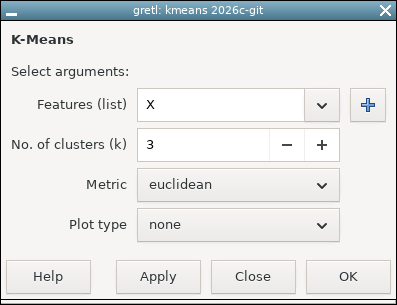
\includegraphics[scale=0.65]{kmeans_dialog.png}
  \caption{K-Means dialog}
  \label{fig:dialog}
\end{figure}

Pulling down the \textsf{Plot type} selector reveals three choices:
``Scree'', ``Cluster (pairs)'' and ``Silhouette''.
\begin{enumerate}
\item In the ``Scree'' case the number of clusters value is taken as a
  maximum, $K^*$ (and you'll probably want to make it larger than the
  default of 3). The $K$-means problem is solved for $K=1,\dots,K^*$ and
  you are shown the relationship between number of clusters and the
  minimized value of within-cluster distance.
\item In the ``Cluster (pairs)'' case you get a grid holding pairwise
  plots of the $n$ features, factorized by their estimated cluster
  membership.
\item In the ``Silhouette'' case you get a plot for each cluster,
  showing the Silhouette score for each point (ranked from best to worst
  in terms of the solidity of its assignment to the cluster) as well as
  the average across all clusters.
\end{enumerate}

\clearpage

\section{Reference: public functions}
\label{sec:funcref}

\begin{funcdoc}
\begin{verbatim}
bundle kmeans_fit (list xlist, numeric clusters, bundle opts[null])
\end{verbatim}
  Executes the $K$-means algorithm and estimates the clusters. The
  \texttt{xlist} argument, which specifies the features on which
  clustering is to be based, must not contain any missing values, so be
  sure to clean your data before calling this function.  The
  \texttt{clusters} argument must be either a positive integer,
  specifying the assumed number of clusters, $K$, or a $K \times n$
  matrix holding initial centroids.  Table~\ref{tab:fit-parms} lists
  the parameters that can be passed via the \texttt{opts} argument.
\end{funcdoc}

\begin{table}[htbp]
  \centering
  \begin{tabular}{llp{0.7\textwidth}}
    \texttt{metric} & string & specifies the distance metric, default
      \texttt{euclidean}. Alternatives includes
      \texttt{manhattan} and \texttt{chebyshev}; see the help for
      gretl's \texttt{distance()} function for a full list. \\
    \texttt{init} & string & TBD \\
    \dtk{n_draws} & scalar & integer specifying how many times the
      $K$-means algorithm will be run with different randomly
      selected initial centroids, default 8. \\
    \texttt{tolerance} & scalar & value for the improvement in
      the objective function below which the algorithm is considered as
      having converged, default 0.0001.\\
    \texttt{verbosity} & scalar & integer governing printed output: 0 means
      don't print anything; 1, print some details; 2, print more details.
  \end{tabular}
  \caption{Summary of optional parameters for \dtk{kmeans_fit}}
  \label{tab:fit-parms}
\end{table}

The bundle returned by \dtk{kmeans_fit} contains the items shown in
Table~\ref{tab:fit-return}.

\begin{table}[htbp]
  \centering
  \begin{tabular}{llp{0.6\textwidth}}
    \dtk{between_distance} & scalar & TBD \\
    \texttt{centroids} & matrix & holds the optimized centroids, $K
                                  \times n$.\\
    \dtk{cluster_id} & matrix & $m$-vector recording for each data-point
                                the cluster to which it is assigned \\
    \texttt{distances} & matrix & $m$-vector recording for each
                                  data-point the distance to its
                                  associated centroid\\
    \texttt{error} & scalar & error code: either 0 for no error
                              or a positive integer.\\
    \texttt{nobs} & scalar & the number of observations used.\\
    \dots & \dots & TBD
  \end{tabular}
  \caption{Members of the bundle returned by \dtk{kmeans_fit}}
  \label{tab:fit-return}
\end{table}

\begin{funcdoc}
\begin{verbatim}
series kmeans_predict (const list xlist, const bundle Model)
\end{verbatim}
  The first argument should be a list of features, as in
  \dtk{kmeans_fit}, and the second should be a bundle obtained from
  \dtk{kmeans_fit}.  The series that is returned holds the predicted
  cluster ID for each observation of \texttt{xlist} in the current
  sample range.
\end{funcdoc}

\begin{funcdoc}
\begin{verbatim}
void kmeans_summary (const bundle Model)
\end{verbatim}
  Prints summary information given a bundle obtained from \dtk{kmeans_fit}.
\end{funcdoc}

\begin{funcdoc}
\begin{verbatim}
void kmeans_plot (const list xlist, const bundle Model)
\end{verbatim}
  Produces a scatter plot for each pair of features in xlist, factorized
  by the \dtk{cluster_id} series in \texttt{Model}

  ... CLARIFY!  self: bundle, Bundle for manipulating the
  plot. [Here you can also pass options accepted by the
  PairPlot package.]
\end{funcdoc}

\begin{funcdoc}
\begin{verbatim}
matrix kmeans_scree (list xlist, int Kmax, bundle opts[null])
\end{verbatim}
  Produces a two-column matrix representing the ``scree'' field for a
  $K$-means problem.  The first column holds number of clusters, from 1
  to \texttt{Kmax}, and the second holds the minimized within-cluster
  distance. The \texttt{opts} bundle can hold options relevant to
  \dtk{kmeans_fit}, which is called multiple times to fill the matrix.
\end{funcdoc}

\begin{funcdoc}
\begin{verbatim}
void kmeans_screeplot (matrix scree, string filename[null], bundle opts[null])
\end{verbatim}
  Produces a so-called scree plot, showing total within-cluster distance
  as a function of the number of assumed clusters, from 1 to some
  maximum value of $K$.  Adding a cluster is bound to reduce
  within-cluster distance, but if the plot shows an ``elbow'' where the
  slope becomes markedly flatter this gives an informal indication of
  the most appropriate number of clusters.

  The first argument should be obtained from \dtk{kmeans_scree}. If the
  second argument is given it should be the name of a file to which
  the graphic should be written (by default it is shown on-screen). The
  last argument \dots TBD
\end{funcdoc}

\begin{funcdoc}
\begin{verbatim}
matrix kmeans_crosstab (series cluster_id, series actual)
\end{verbatim}
  Relevant only if the dataset in use contains a series which identifies
  underlying clusters, for example the \texttt{species} series in the
  iris dataset (\texttt{iris.gdt}). It can then be of interest to see
  the degree of match between the clusters obtained via the $K$-means
  algorithm (\dtk{cluster_id}) and the underlying ones (generically,
  \texttt{actual}). Since the numeric coding of the clusters is
  essentially arbitrary, a simple cross-tabulation is likely to show
  garbled results. This function searches for the most appropriate
  mapping between the estimated clusters and the ``actual'' ones,
  defined as that which maximizes the number of matched observations
  (the trace of the cross-tabulation). The crosstab is printed using
  gretl's \texttt{xtab} command, and is also returned in matrix form.
\end{funcdoc}

%% WORK needed below here!!

\bibliographystyle{gretl}
\bibliography{gretl}

\end{document}

\begin{funcdoc}
\begin{verbatim}
kmeans_screeplot (list xlist, int Kmax, string filename[null], bundle self[null])
\end{verbatim}
  This function produces a so-called scree plot for the $K$-means
  algorithm. The plot shows total within-cluster distance as a
  function of the number of assumed clusters, from 1 to \texttt{Kmax}.
  Adding a cluster is bound to reduce within-cluster distance, but if
  the plot shows an ``elbow'' where the slope becomes markedly flatter
  this gives an informal indication of the most appropriate number of
  clusters.
\end{funcdoc}

**screeplotArguments:**

- `xlist`: list, Features (regressors) used for plotting.
- `max_clusters`: int, Maximum number of clusters to plot (default: 3).
- `filename`: string, Name of the file to save the plot (optional). If not provided, the plot will be shown on the screen.
- `self`: bundle, Bundle for manipulating the plot (optional). **Note, accepted options are:**

    * The same as for the `kmeans_fit()` function for the `opts` bundle. Relevant for controlling the k-means algorithm.
    * `verbose`: int, If `2` show summary for each model, else show nothing.
    * `fontsize`: scalar, Font size for the plot.
    * `linewidth`: scalar, Line width for the plot.

**Return:** Matrix with two columns: the first column is the number of clusters, and the second column is the within-cluster sum of squares (*inertia*). Each row corresponds to a different number of clusters.


## kmeans_sil_samples

```
kmeans_sil_samples (bundle Model, list xlist)
```

Compute the silhouette sample value for each observation in the fitted
kmeans model. The silhouette value measures how similar an observation
is to its own cluster compared to other clusters.

**Reference:** https://en.wikipedia.org/wiki/Silhouette_(clustering)

**Arguments:**

- `Model`: bundle, Model object returned by the `kmeans_fit()` function.
- `xlist`: list, Features (regressors) used for clustering.

**Return:** Series holding the silhouette value for each observation.


## kmeans_sil_score

```
kmeans_sil_score (bundle Model, list xlist, bool global[TRUE])
```

Compute the mean silhouette score for all samples in the fitted kmeans
model if the optional parameter `global` is set to `TRUE` (default). The
silhouette score is a measure of how well clusters are separated; higher
values indicate better-defined clusters. The best value is 1 and the
worst value is -1. Values near 0 indicate overlapping clusters. Negative
values generally indicate that a sample has been assigned to the wrong
cluster, as a different cluster is more similar. If `global` is set to
`FALSE`, the mean silhouette score is computed for each cluster
separately.

**Reference:** https://scikit-learn.org/stable/modules/generated/sklearn.metrics.silhouette_score.html

**Arguments:**

- `Model`: bundle, Model object returned by the `kmeans_fit()` function.
- `xlist`: list, Features (regressors) used for clustering.
- `global`: bool, If TRUE (default) compute the mean silhouette score for all samples, otherwise compute it for each cluster separately.

**Return:** Scalar value representing the mean silhouette score if `global` is set to TRUE, otherwise a matrix is returned  (columns refer to the cluster and the score).


## kmeans_sil_plot

```
kmeans_sil_plot (bundle Model, list xlist, bundle opts[null])
```

Create a silhouette plot for the fitted kmeans model. Each cluster is
plotted separately, showing the silhouette value for each
observation. Plot options can be passed via the `opts` bundle. The
dashed vertical line shows the mean Silhouette score.

**Reference:** https://en.wikipedia.org/wiki/Silhouette_(clustering)

**Arguments:**

- `Model`: bundle, Model object returned by the `kmeans_fit()` function.
- `xlist`: list, Features (regressors) used for clustering.
- `opts`: bundle, Optional parameters for controlling the plot. The following options are supported:
    * `filename`: string, Name of the file to save the plot. If not provided, the plot will be shown on the screen.
    * `width`: scalar, Width of the plot in pixels (default: 600).
    * `height`: scalar, Height of the plot in pixels (default: 900).
    * `columns`: scalar, Number of columns in the grid layout for clusters (default: 1).
    * `base_margin`: scalar, Base margin for top and bottom plot margins (default: 2.5).
    * `pointsize`: scalar, Size of points (default: 0.75)

**Return:** Nothing.


\section{Changelog}

* **v0.6 (August 2025)**
    * Add new silhouette functions: `kmeans_sil_samples()`, `kmeans_sil_score()`, and `kmeans_sil_plot()`
    * Bugifx: Correctly handle the case for the "mahalanobis" distance metric in the `compute_distance()` function. (Kudos to Allin Cottrell for reporting and providing a fix)
    * GUI dialog: Add option to plot silhouette analysis and general improvements
    * Raise minimum version of gretl to 2023c

* **v0.5 (February 2025)**
    * Bugfix: in case of a single cluster, switch to "random" initializer as "pca" would fail; throw error if pca initializer is called for a single cluster
    * Improvement: Improve robustness if empty clusters are estimated (e.g., due to bad random initialization of centroids)

* **v0.4 (January 2025)**
    * Add the function `kmeans_screeplot()` for plotting the scree plot (method to determine the optimal number of clusters).
    * Change default values for parameters `pointsize` and `fontsize` in the `kmeans_plot()` function. Now set by gretl's default values.
    * Bugfix: The distance measure is now taken into account when calling the function via the GUI. Before, the default distance measure was always used.

* **v0.3 (February 2024)**
    * Add GUI dialog
    * Move to markdown-based help file
    * Internal improvements

* **v0.2 (July 2022)**
    * Fix bug that arises if the sample range is restricted, and you're trying to coerce a column vector that's not the full length of the dataset into a series on adding it to a bundle.
    * Returned objects `cluster_id` and `distances` when calling the `kmeans_fit()` function are of type matrix instead of series, now.

* **v0.1 (February 2022)**
    * initial release

\end{document}